\chapter{Конструкторский раздел}

В данном разделе будут приведены требования к входным, выходным параметрам и представлены схемы для:
\begin{itemize}[label=--]
    \item рекурсивного алгоритма нахождения расстояния Левенштейна;
    \item рекурсивного алгоритма нахождения расстояния Левенштейна с мемоизацией;
    \item матричного алгоритма нахождения расстояния Левенштейна;
    \item матричного алгоритма нахождения расстояния Дамерау~---~Левенштейна.
\end{itemize}

\section{Требования к входным и выходным параметрам}

Требования к входным и выходным параметрам:
\begin{itemize}[label=--]
    \item в качестве входных параметров программа принимает две строки;
    \item символы разных регистров считаются различными;
    \item пустая строка является корректным входным значением;
    \item выходным параметром является число --- расстояние Левенштейна или Дамерау~---~Левенштейна в зависимости от выбранного алгоритма.
\end{itemize}

\section{Рекурсивный алгоритм Левенштейна}

На рисунке~\ref{fig:recur_lev} представлена схема рекурсивного алгоритма нахождения расстояния Левенштейна.

\begin{figure}[H]
\centering
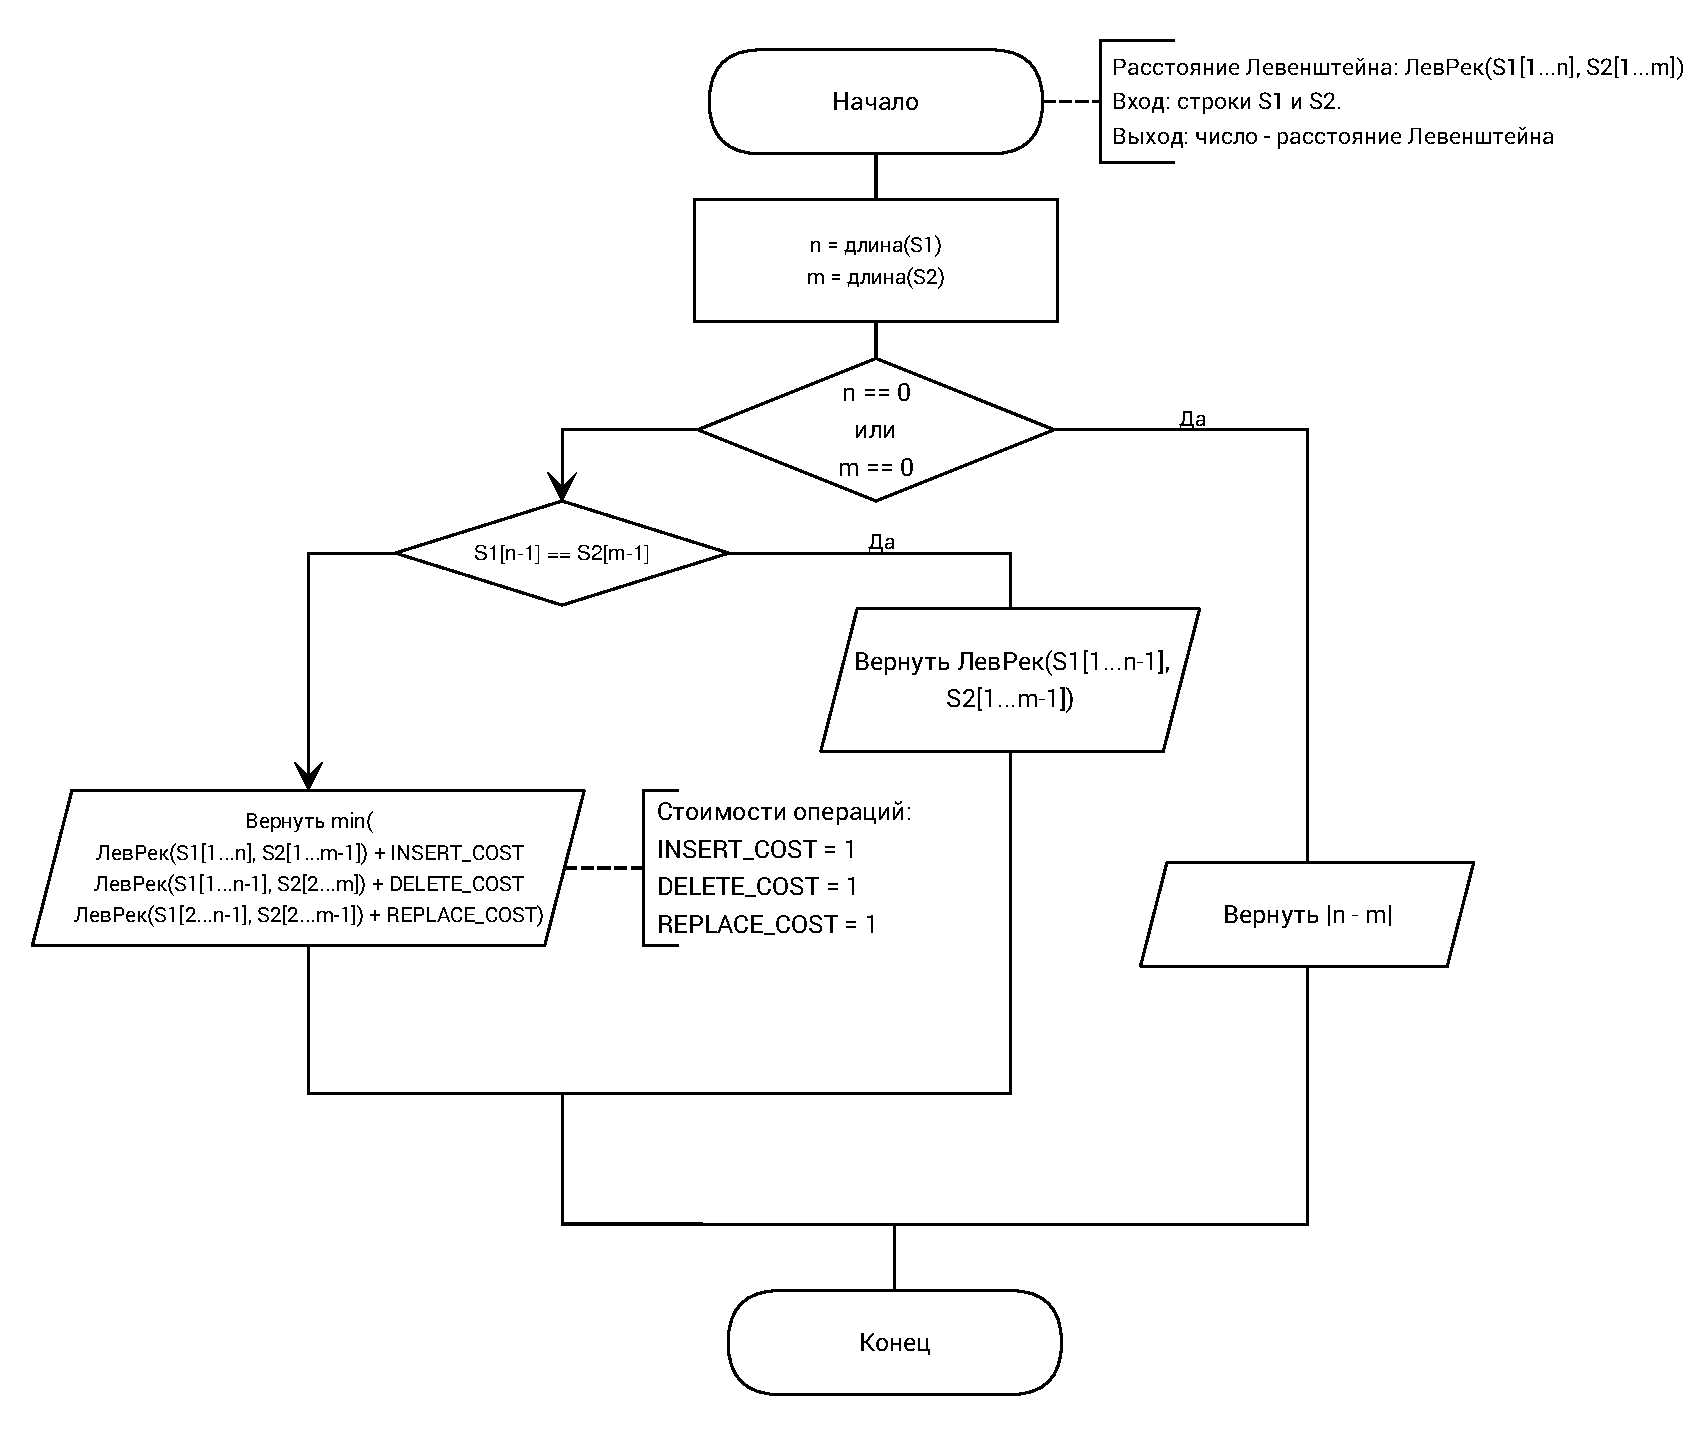
\includegraphics[width=\textwidth]{inc/img/recursive_levenshtein.pdf}
\caption{Схема рекурсивного алгоритма нахождения расстояния \newline Левенштейна}
\label{fig:recur_lev}
\end{figure}

\section{Рекурсивный алгоритм Левенштейна c кэшем}

На рисунке~\ref{fig:recur_lev_cache} представлена схема рекурсивного алгоритма нахождения расстояния Левенштейна c мемоизацией.

\begin{figure}[H]
\centering
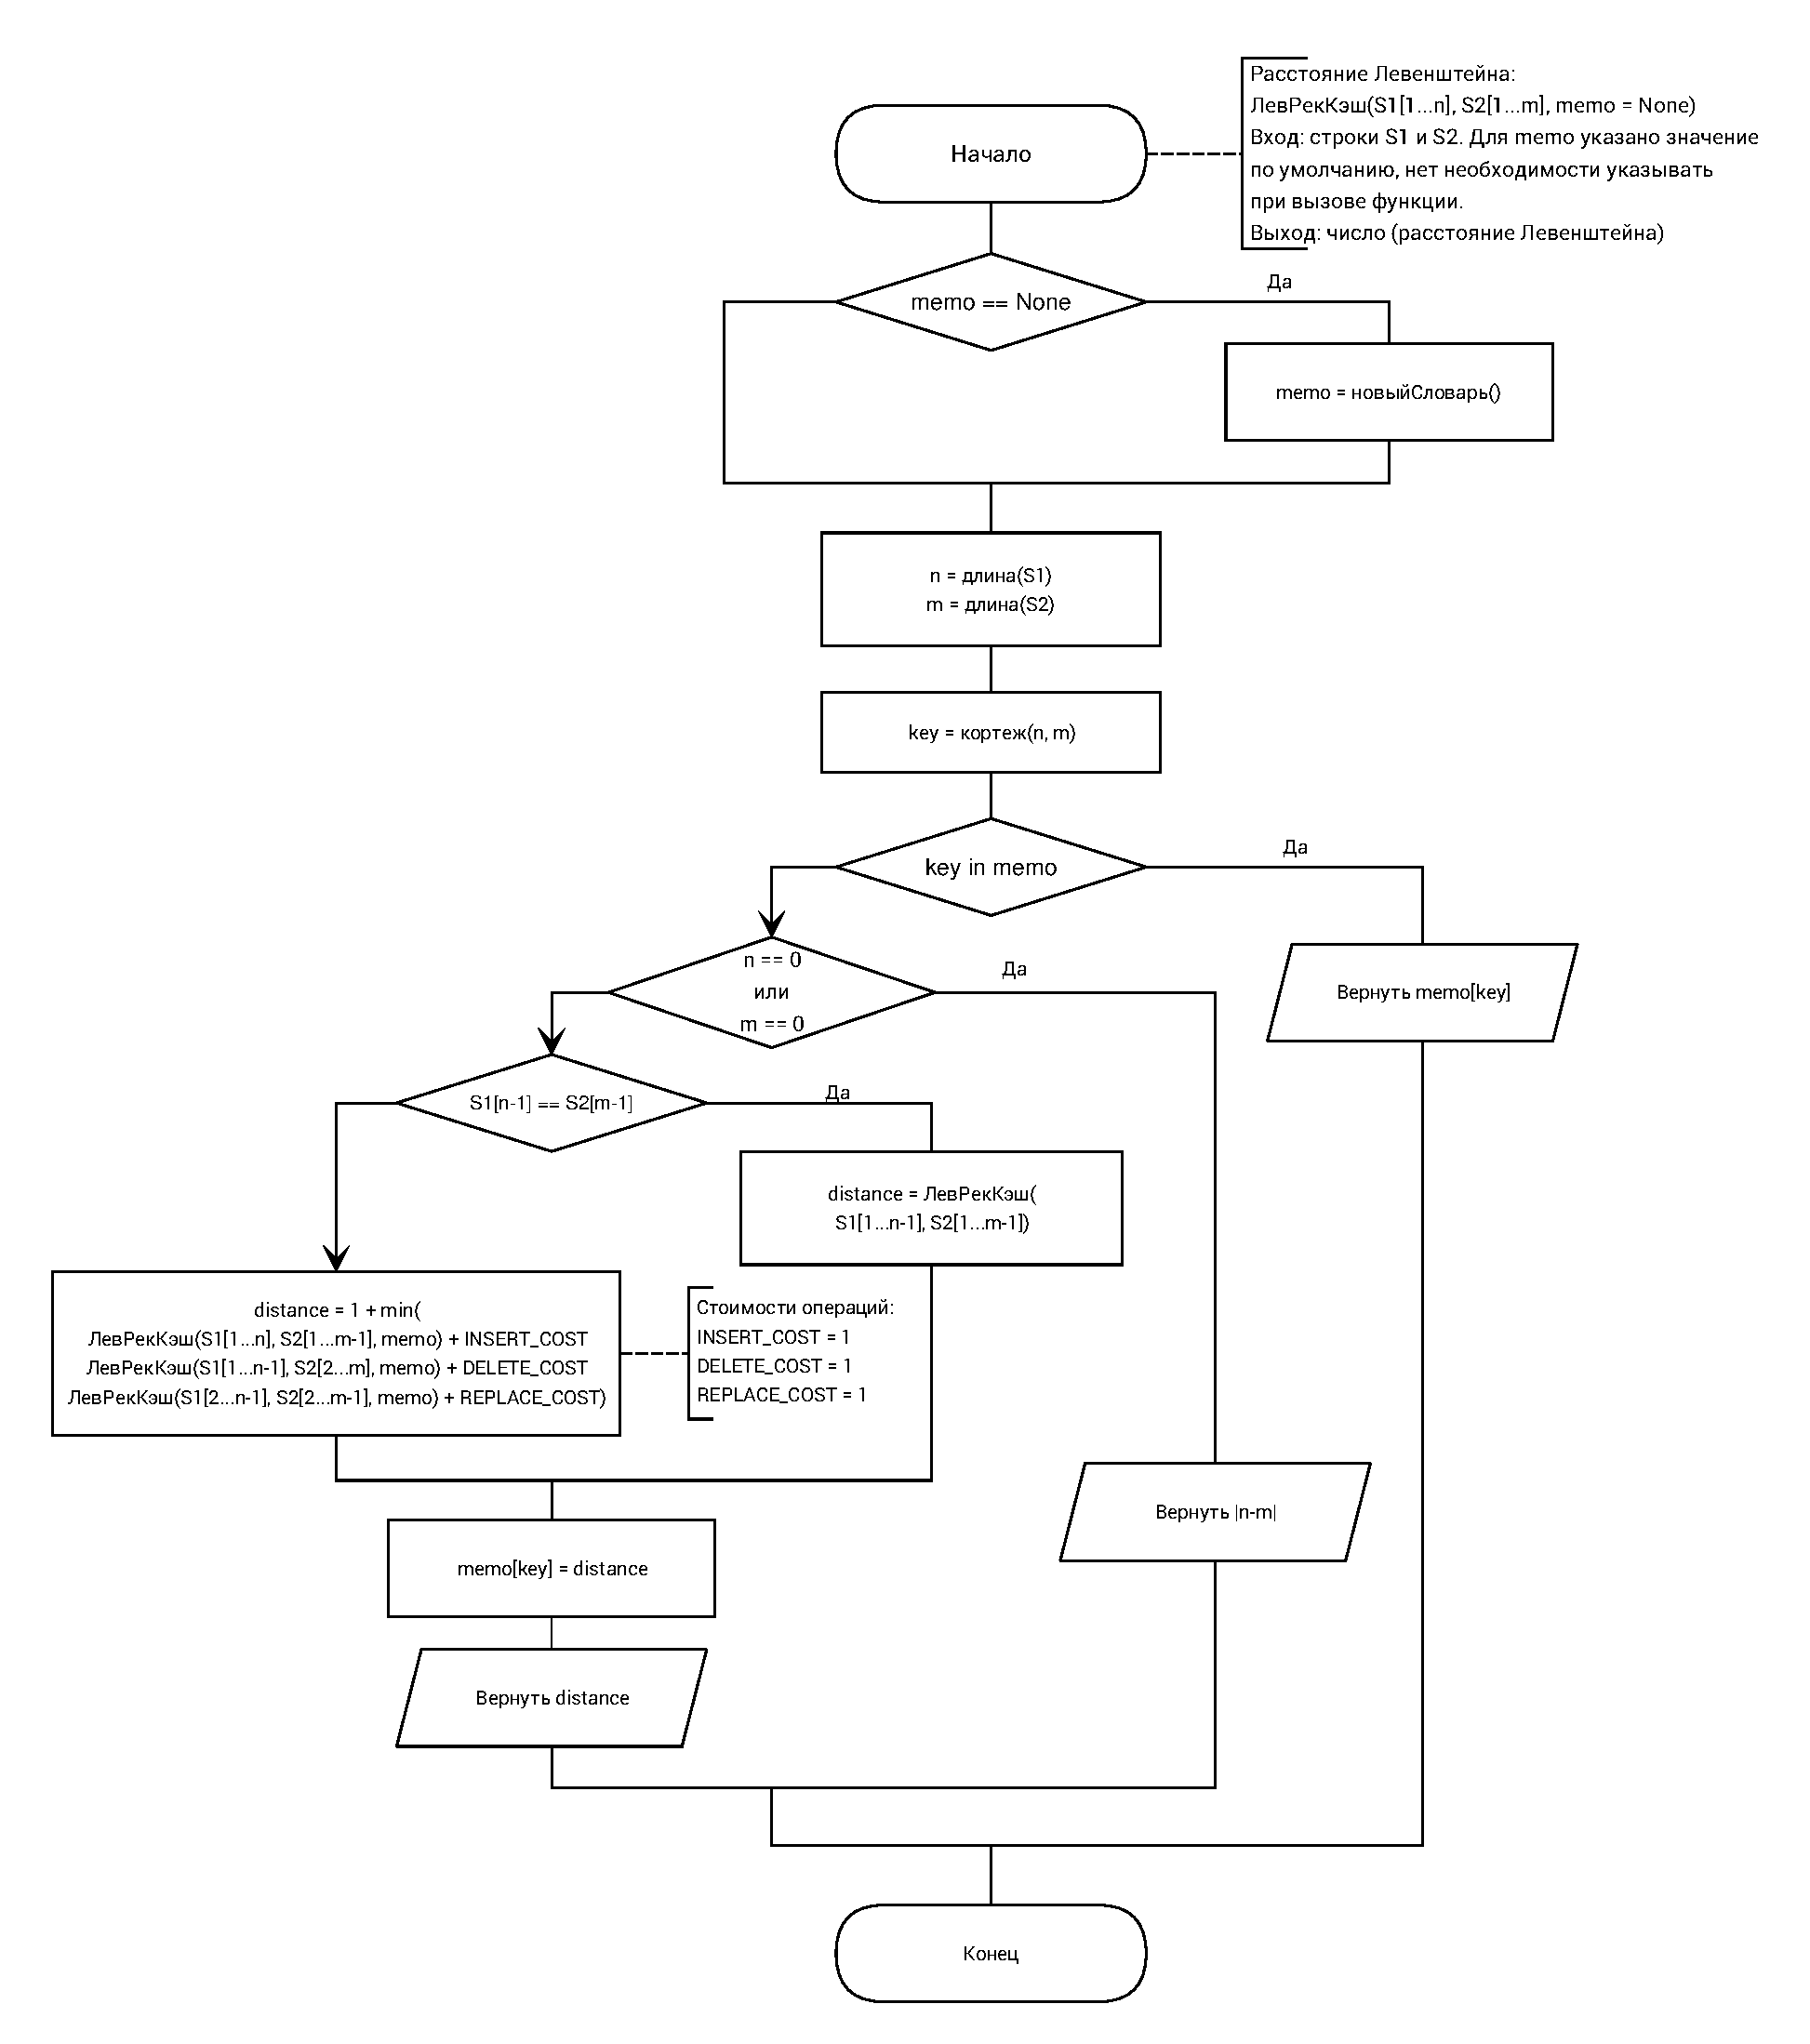
\includegraphics[width=\textwidth]{inc/img/recursive_cache_levenshtein.pdf}
\caption{Схема рекурсивного алгоритма нахождения расстояния Левенштейна с мемоизацией}
\label{fig:recur_lev_cache}
\end{figure}

\section{Матричный алгоритм Левенштейна}

На рисунке~\ref{fig:dyn_lev} представлена схема матричного алгоритма нахождения расстояния Левенштейна.

\begin{figure}[H]
\centering
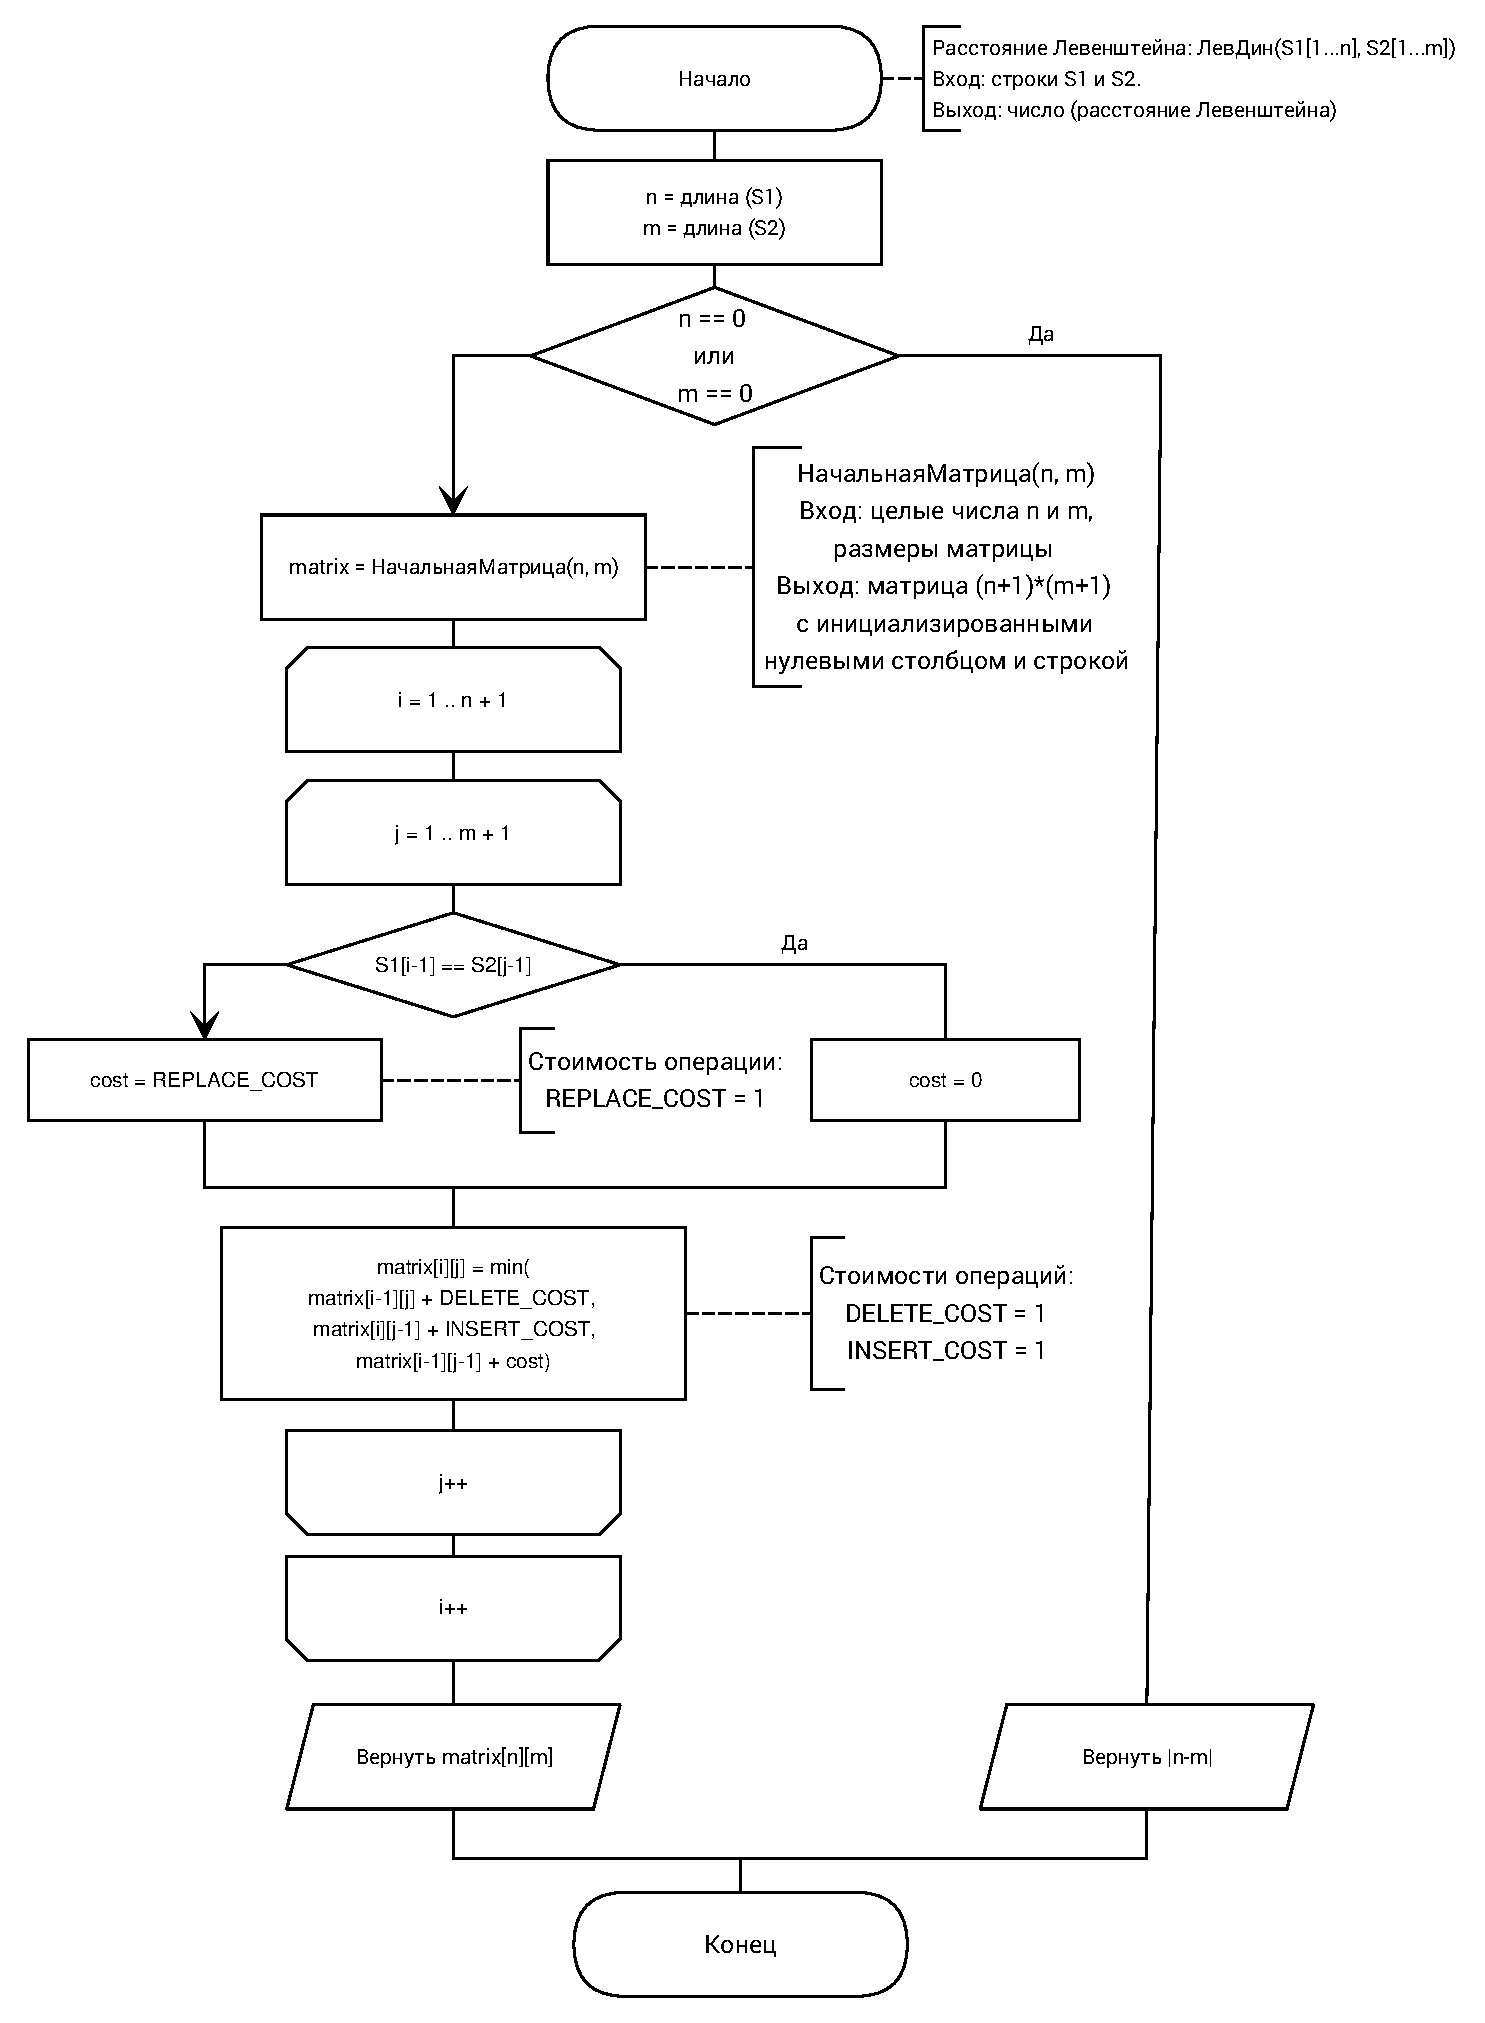
\includegraphics[width=\textwidth]{inc/img/levenshtein_dynamic.pdf}
\caption{Схема матричного алгоритма нахождения расстояния Левенштейна}
\label{fig:dyn_lev}
\end{figure}


\section{Матричный алгоритм Дамерау~---~Левенштейна}

На рисунке~\ref{fig:dyn_dam_lev} представлена схема матричного алгоритма нахождения расстояния Дамерау~---~Левенштейна.

\begin{figure}[H]
\centering
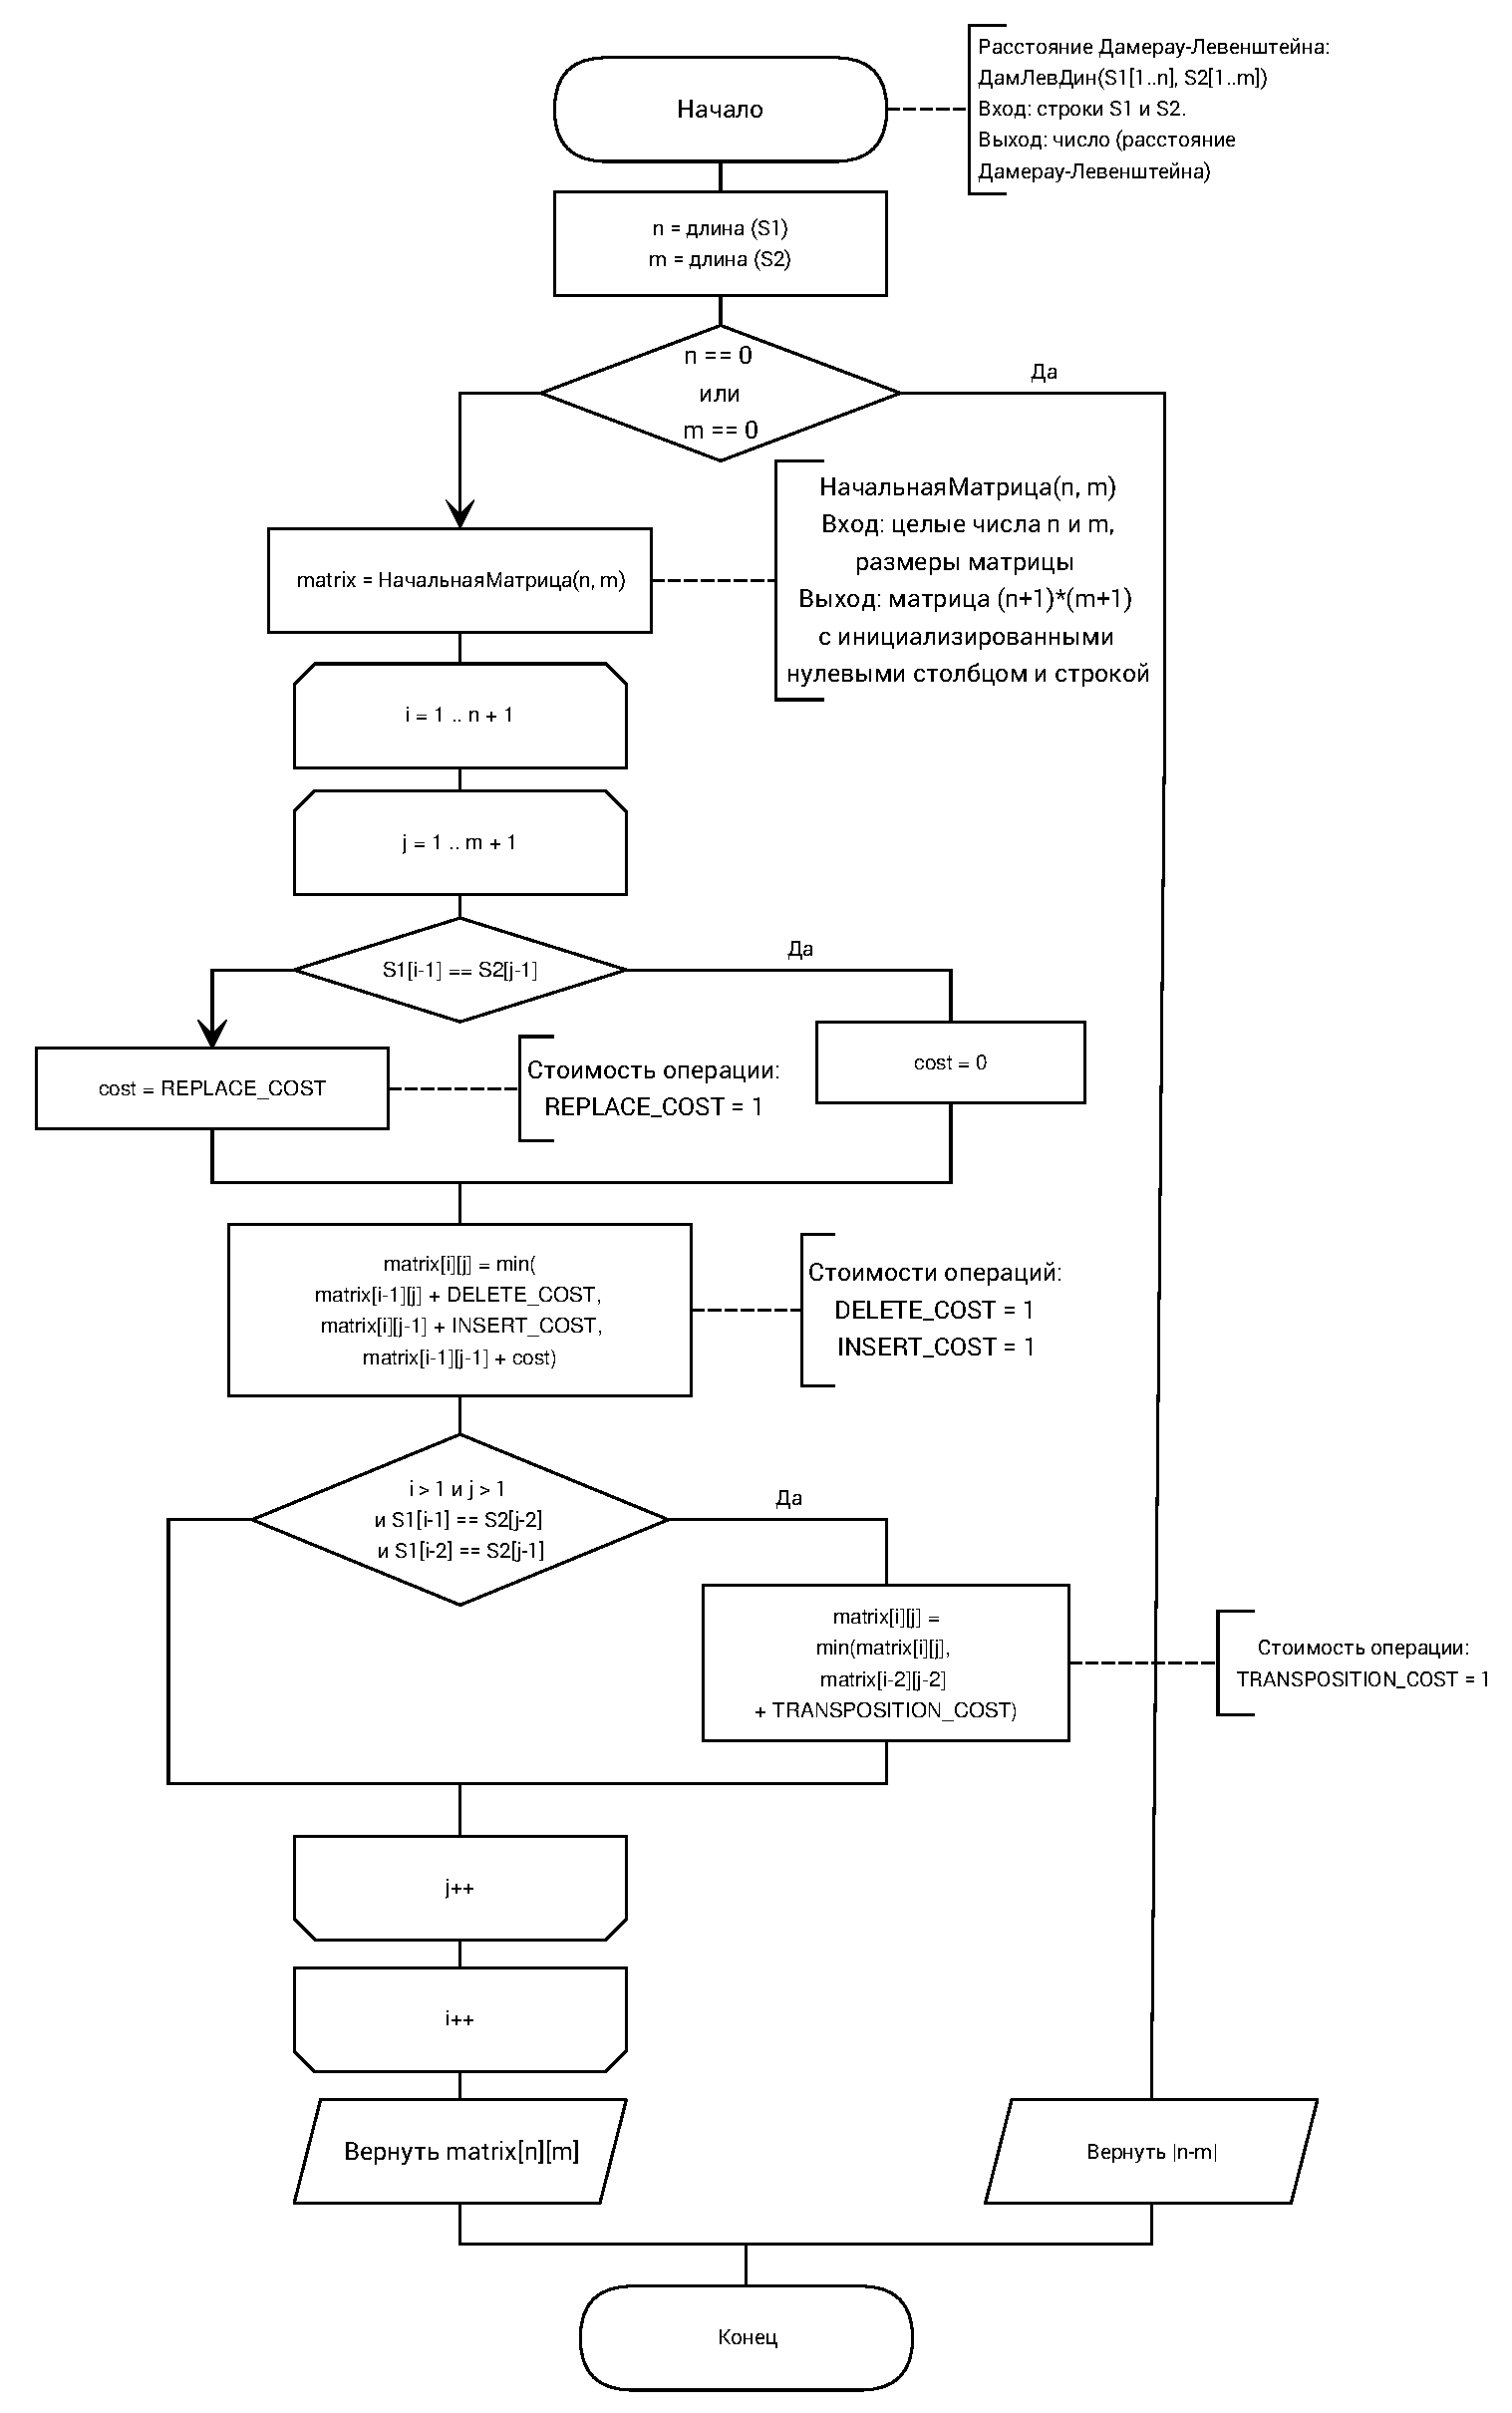
\includegraphics[width=0.85\textwidth]{inc/img/damerau_levenshtein_dynamic.pdf}
\caption{Схема матричного алгоритма нахождения расстояния Дамерау~---~Левенштейна}
\label{fig:dyn_dam_lev}
\end{figure}

